\newpage
\appendix %Appendix begin
\section{Appendix}
\subsection{Orchestrator.sh} \label{orchestrator_appendix}
\begin{minted}[fontsize=\small, bgcolor=gray!5, frame=lines, linenos]{bash}
#!/bin/bash

set -e

ENV_FILE=".env"

SCRIPT_DIR="$(cd "$(dirname "${BASH_SOURCE[0]}")" && pwd)"

if [ ! -f "$SCRIPT_DIR/$ENV_FILE" ] || [ ! -r "$SCRIPT_DIR/$ENV_FILE" ]; then
    echo "Error: $ENV_FILE not found or not readable in $SCRIPT_DIR"
    exit 1
fi

# Load all variables from .env
while IFS='=' read -r key value; do
    if [[ -n "$key" && ! "$key" =~ ^# ]]; then
        key=$(echo "$key" | tr -d '[:space:]')
        value=$(echo "$value" | tr -d '[:space:]')
        eval "export $key=$value"
    fi
done < "$SCRIPT_DIR/$ENV_FILE"

# Verify required IP variables
REQUIRED_IPS=("REGISTRY_IP" "GATEWAY_IP" "BAP_IP" "BPP_IP")
for var in "${REQUIRED_IPS[@]}"; do
    if [ -z "${!var}" ]; then
        echo "Error: Required variable $var is not set in $ENV_FILE"
        exit 1
    fi
done

SERVERS=(
    "$REGISTRY_IP"
    "$GATEWAY_IP"
    "$BAP_IP"
    "$BPP_IP"
)

run_script_on_all() {
    local script=$1
    echo "Running $script on all servers..."

    pids=()
    for server in "${SERVERS[@]}"; do
        env_vars=$(while IFS='=' read -r key value; do
            if [[ -n "$key" && ! "$key" =~ ^# ]]; then
                key=$(echo "$key" | tr -d '[:space:]')
                value=$(echo "$value" | tr -d '[:space:]')
                printf '%s=%q ' "$key" "$value"
            fi
        done < "$SCRIPT_DIR/$ENV_FILE")
        
        ssh -o StrictHostKeyChecking=no root@"$server" "export $env_vars \
        CURRENT_SERVER=$server; bash -s" < "$SCRIPT_DIR/$script" &
        pids+=($!)
    done

    # Wait for all background jobs to finish and check results
    failures=0
    for i in "${!pids[@]}"; do
        pid=${pids[$i]}
        server=${SERVERS[$i]}
        if wait "$pid"; then
            echo "Success: $script completed on $server"
        else
            echo "Failure: $script failed on $server"
            failures=$((failures + 1))
        fi
    done

    if [ "$failures" -ne 0 ]; then
        echo "Error: $script failed on $failures server(s)"
        exit 1
    fi

    echo "$script completed successfully on all servers."
}

run_local_script() {
    local script=$1
    echo "Running $script locally..."
    if bash "$SCRIPT_DIR/$script"; then
        echo "Success: $script completed locally"
    else
        echo "Failure: $script failed locally"
        exit 1
    fi
}

run_script_on_server() {
    local script=$1
    local server=$2
    echo "Running $script on $server..."

    env_vars=$(while IFS='=' read -r key value; do
        if [[ -n "$key" && ! "$key" =~ ^# ]]; then
            key=$(echo "$key" | tr -d '[:space:]')
            value=$(echo "$value" | tr -d '[:space:]')
            printf '%s=%q ' "$key" "$value"
        fi
    done < "$SCRIPT_DIR/$ENV_FILE")

    if ssh -o StrictHostKeyChecking=no root@"$server" "export $env_vars \
    CURRENT_SERVER=$server; bash -s" < "$SCRIPT_DIR/$script"; then
        echo "Success: $script completed on $server"
    else
        echo "Failure: $script failed on $server"
        exit 1
    fi
}

# Define the ordered list of scripts and their type (local, remote or server)
TASKS=(
    "setup_docker.sh:remote"
    "install_nginx.sh:remote"
    "nginx-configs/generate_all_configs.sh:local"
    "nginx-configs/upload_nginx_configs.sh:local"
    "nginx-configs/deploy_enable_configs.sh:remote"
    "setup_tls.sh:remote"
    "clone_repo.sh:remote"
    "start_webhook.sh:server:$BPP_IP"
    "beckn_setup/setup_registry.sh:server:$REGISTRY_IP"
    "beckn_setup/setup_registry.sh:server:$REGISTRY_IP"
    "beckn_setup/setup_gateway.sh:server:$GATEWAY_IP"
    "beckn_setup/setup_bap.sh:server:$BAP_IP"
    "beckn_setup/setup_bpp.sh:server:$BPP_IP"
    "beckn_setup/bap_layer2.sh:server:$BAP_IP"
    "beckn_setup/bpp_layer2.sh:server:$BPP_IP"
)

for task in "${TASKS[@]}"; do
    IFS=':' read -r script type server <<< "$task"
    case "$type" in
        remote)
            run_script_on_all "$script"
            ;;
        local)
            run_local_script "$script"
            ;;
        server)
            run_script_on_server "$script" "$server"
            ;;
        *)
            echo "Unknown task type: $type for script: $script"
            exit 1
            ;;
    esac
done

echo "All scripts completed successfully on all servers!"
\end{minted}
\subsection{Logbook} \label{logbook_appendix}
This appendix contains screenshots of the weekly logbooks maintained during the project. Each entry corresponds to a specific week or part of a week and is presented as an image.


\begin{figure}[H]
    \centering
    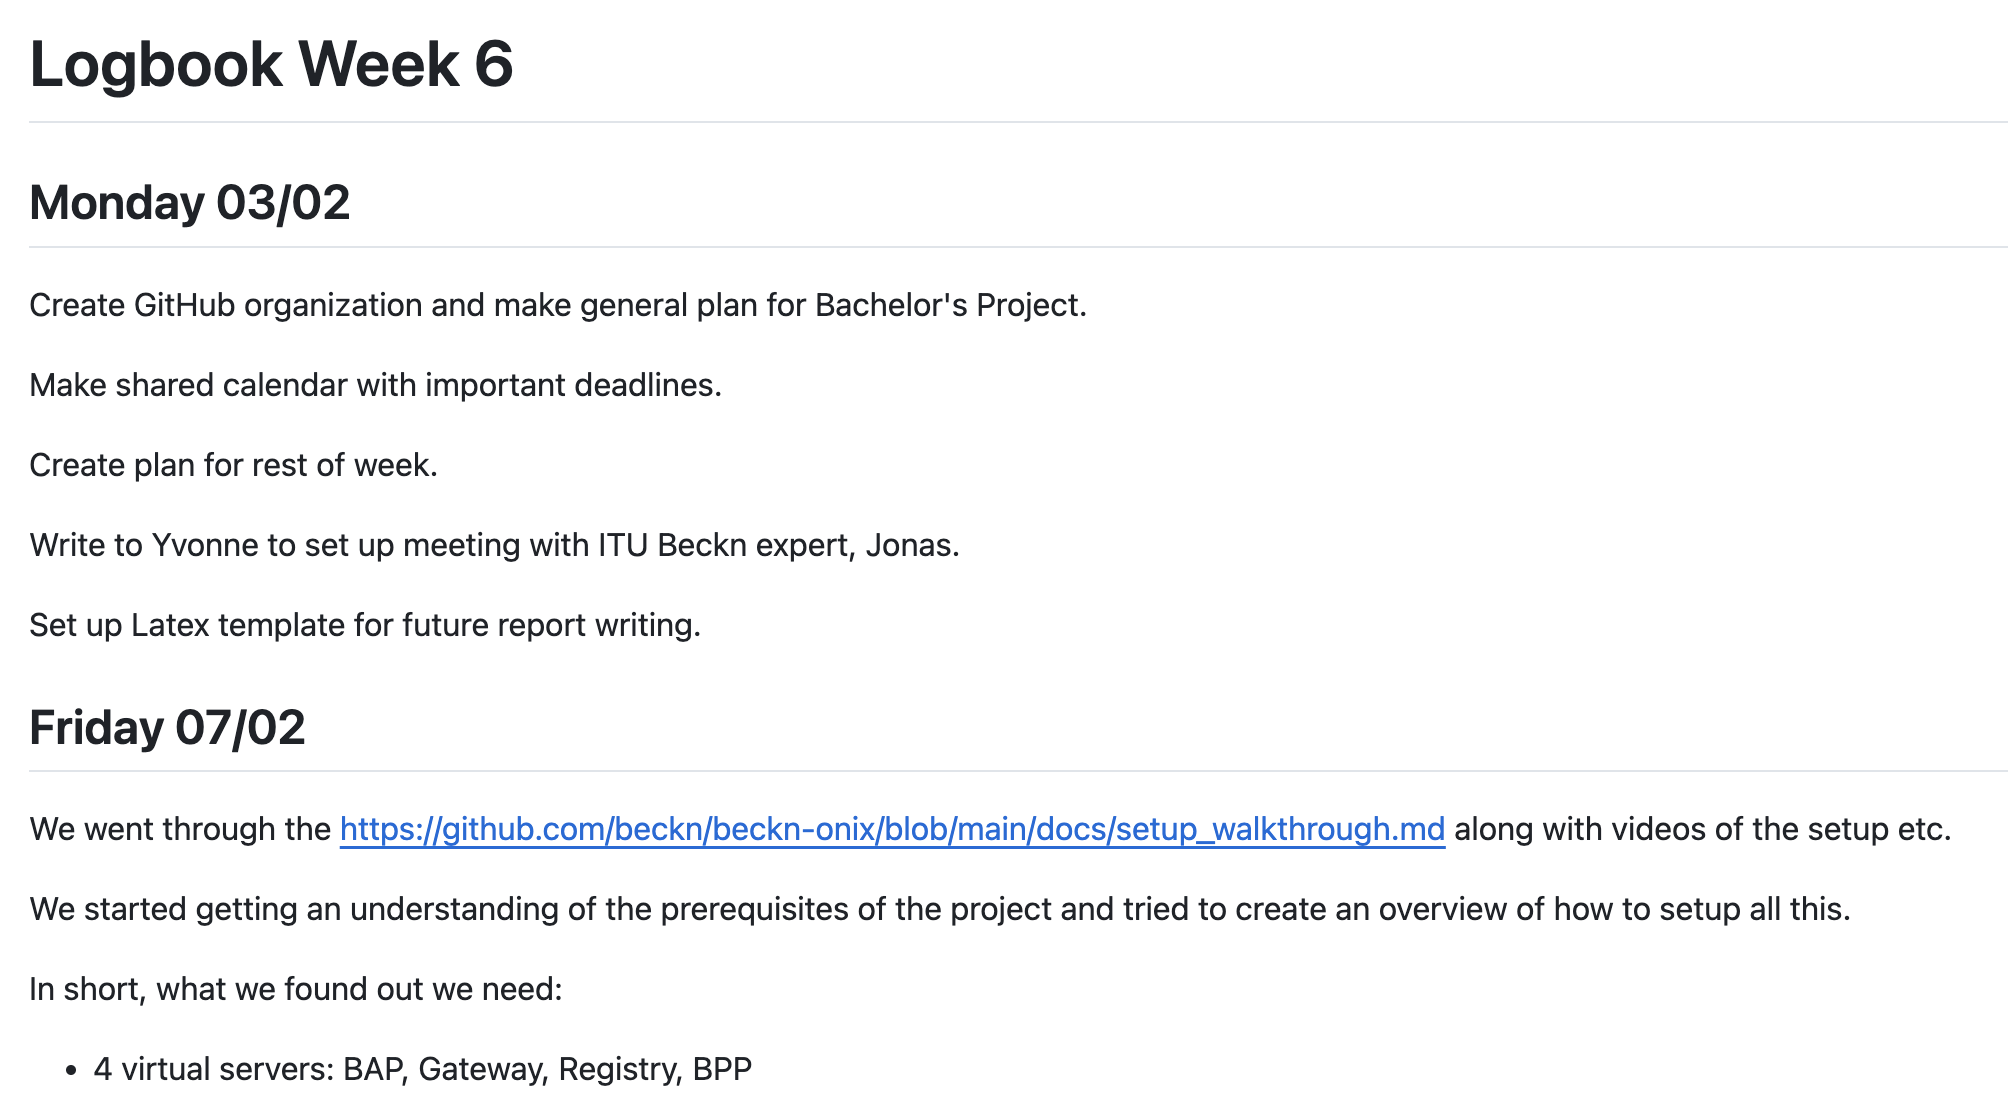
\includegraphics[width=\textwidth]{Images/week_6.1.png}
\end{figure}


\begin{figure}[H]
    \centering
    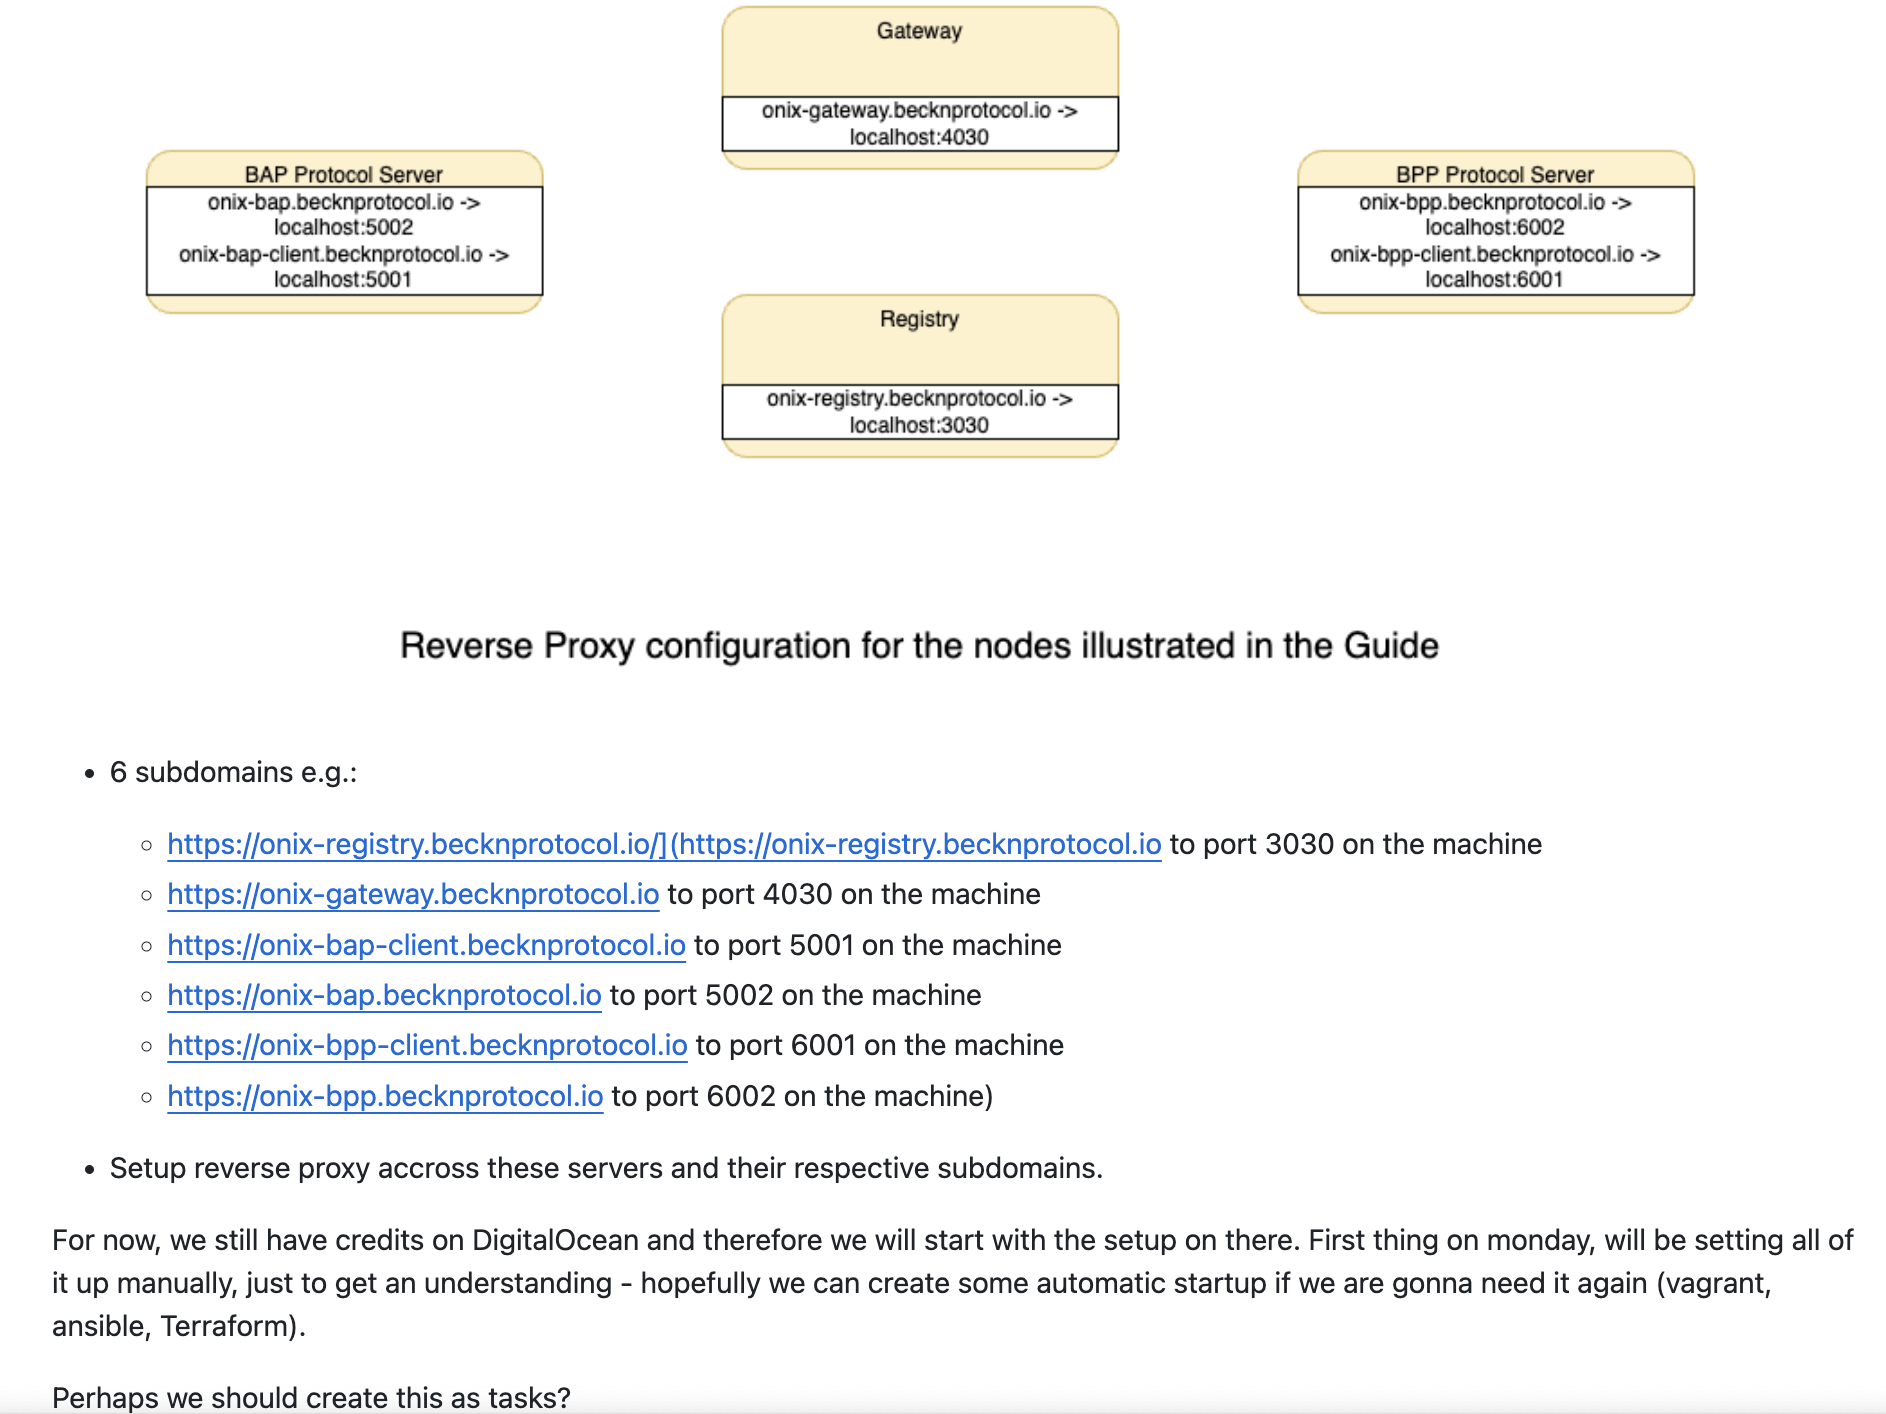
\includegraphics[width=\textwidth]{Images/week_6.2.png}
\end{figure}

\clearpage
\begin{figure}[H]
    \centering
    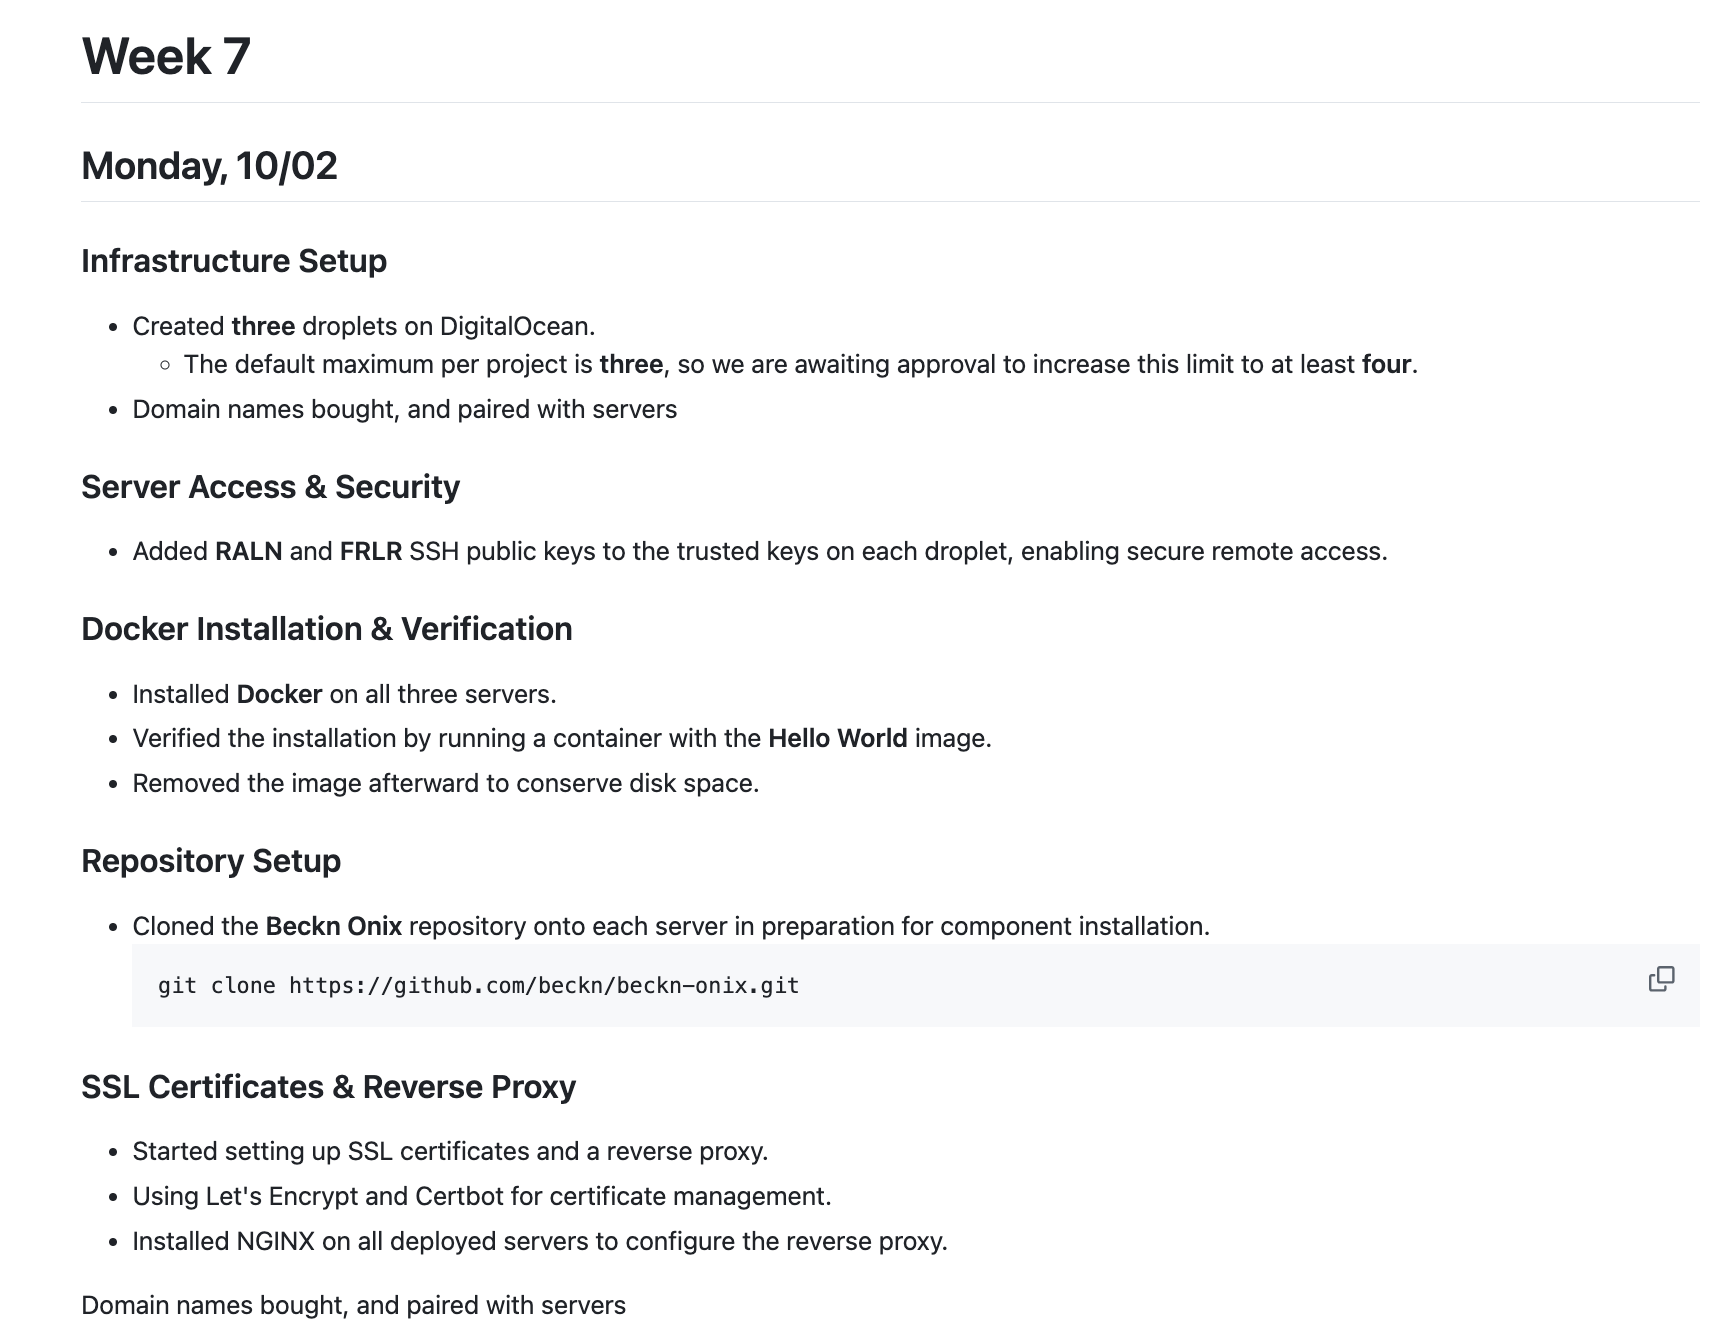
\includegraphics[width=\textwidth]{Images/week_7.1.png}
\end{figure}

\begin{figure}[H]
    \centering
    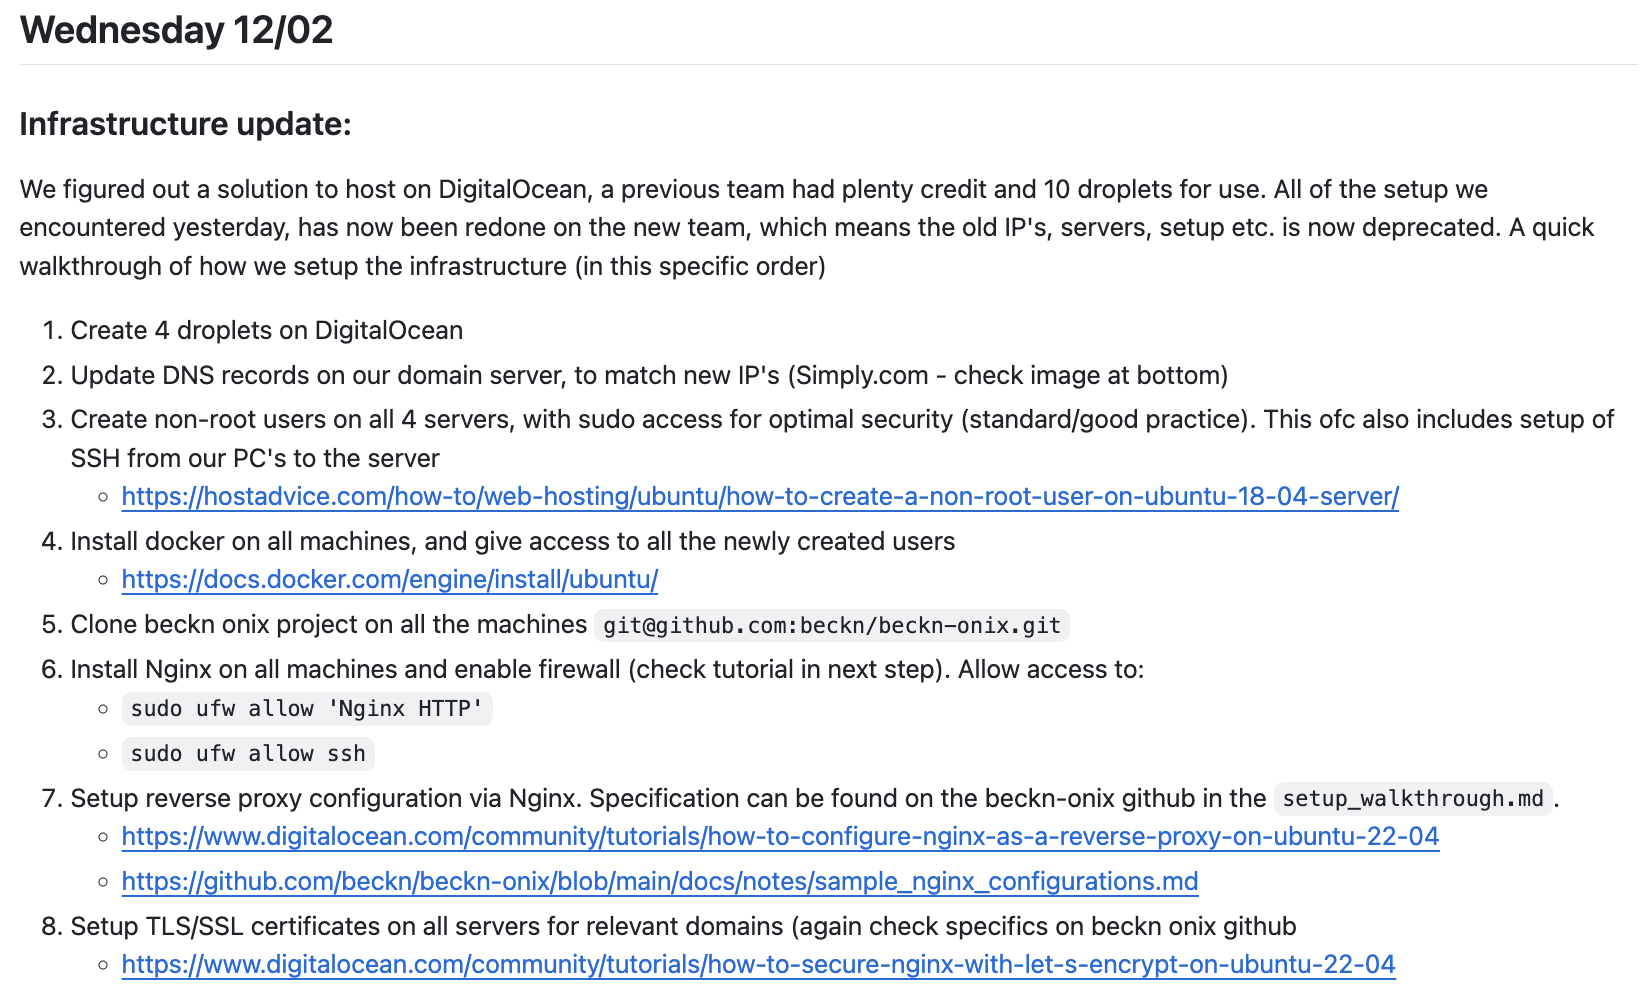
\includegraphics[width=\textwidth]{Images/week_7.2.png}
\end{figure}

\begin{figure}[H]
    \centering
    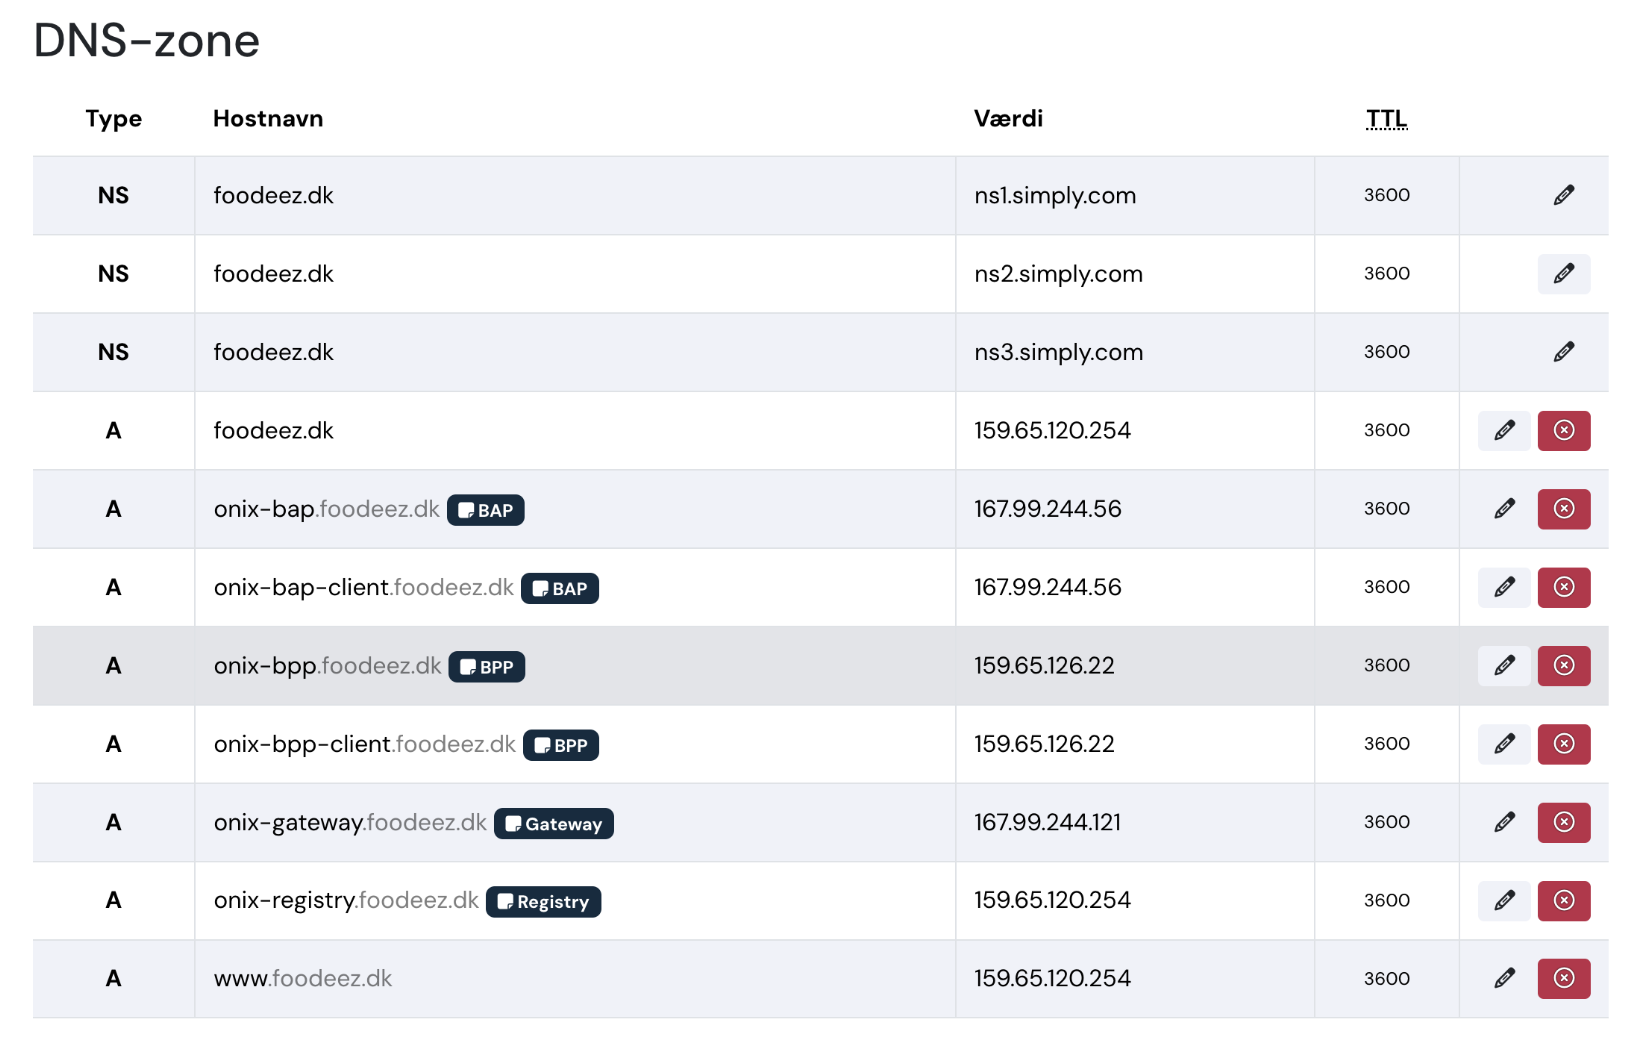
\includegraphics[width=\textwidth]{Images/week_7.3.png}
\end{figure}

\begin{figure}[H]
    \centering
    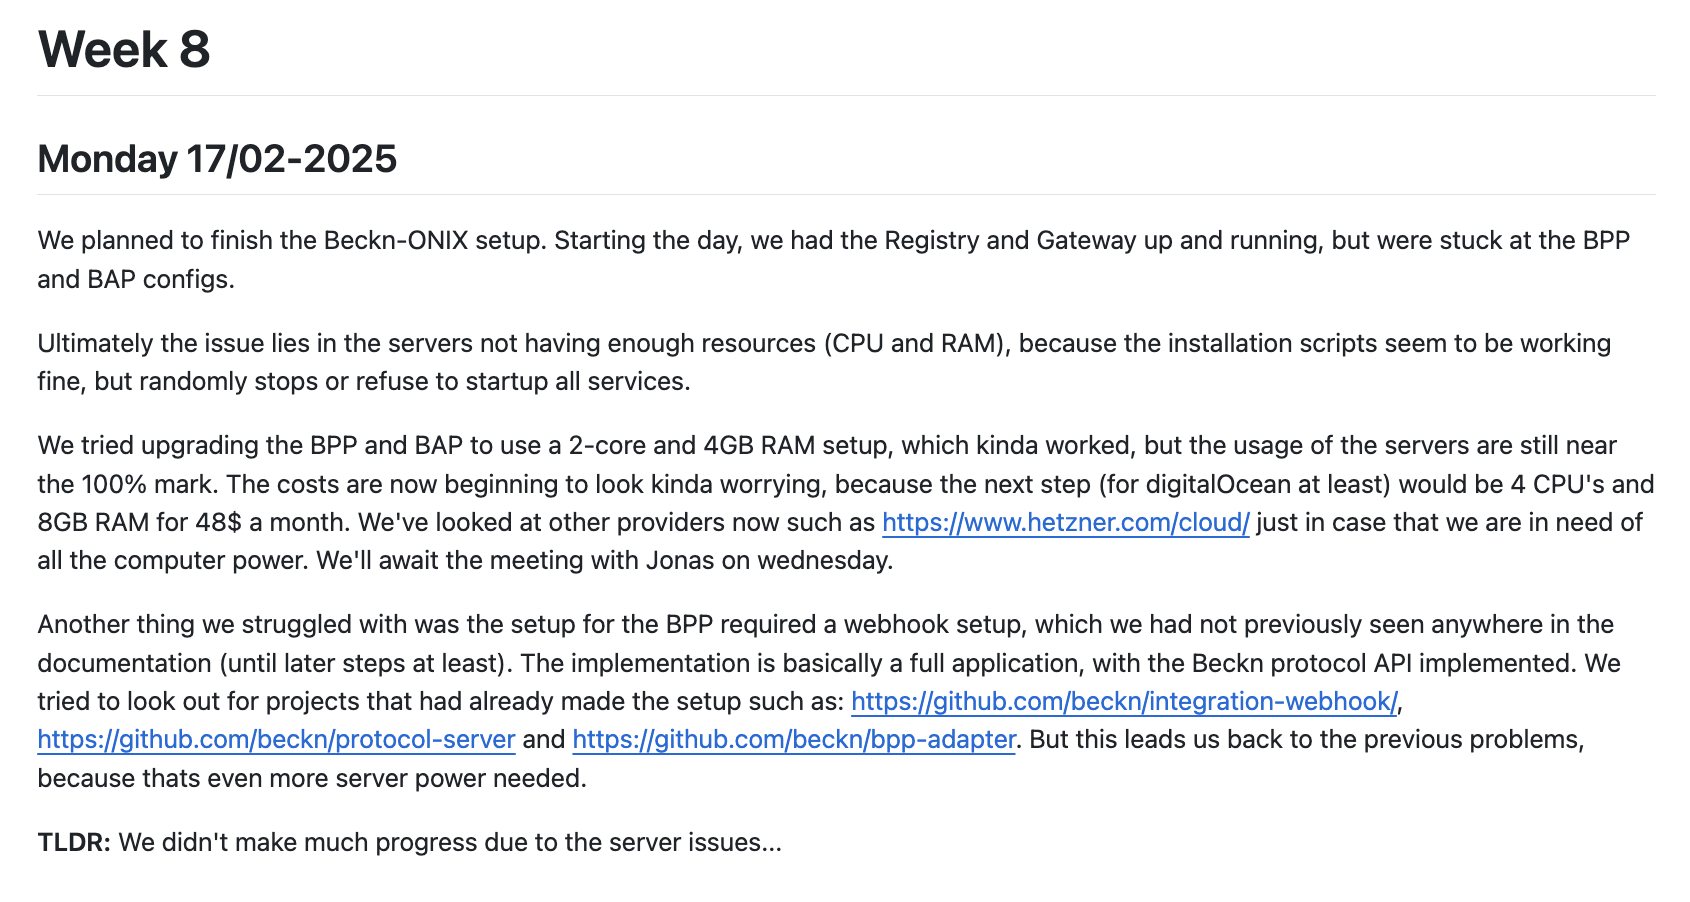
\includegraphics[width=\textwidth]{Images/week_08.png}
\end{figure}

\begin{figure}[H]
    \centering
    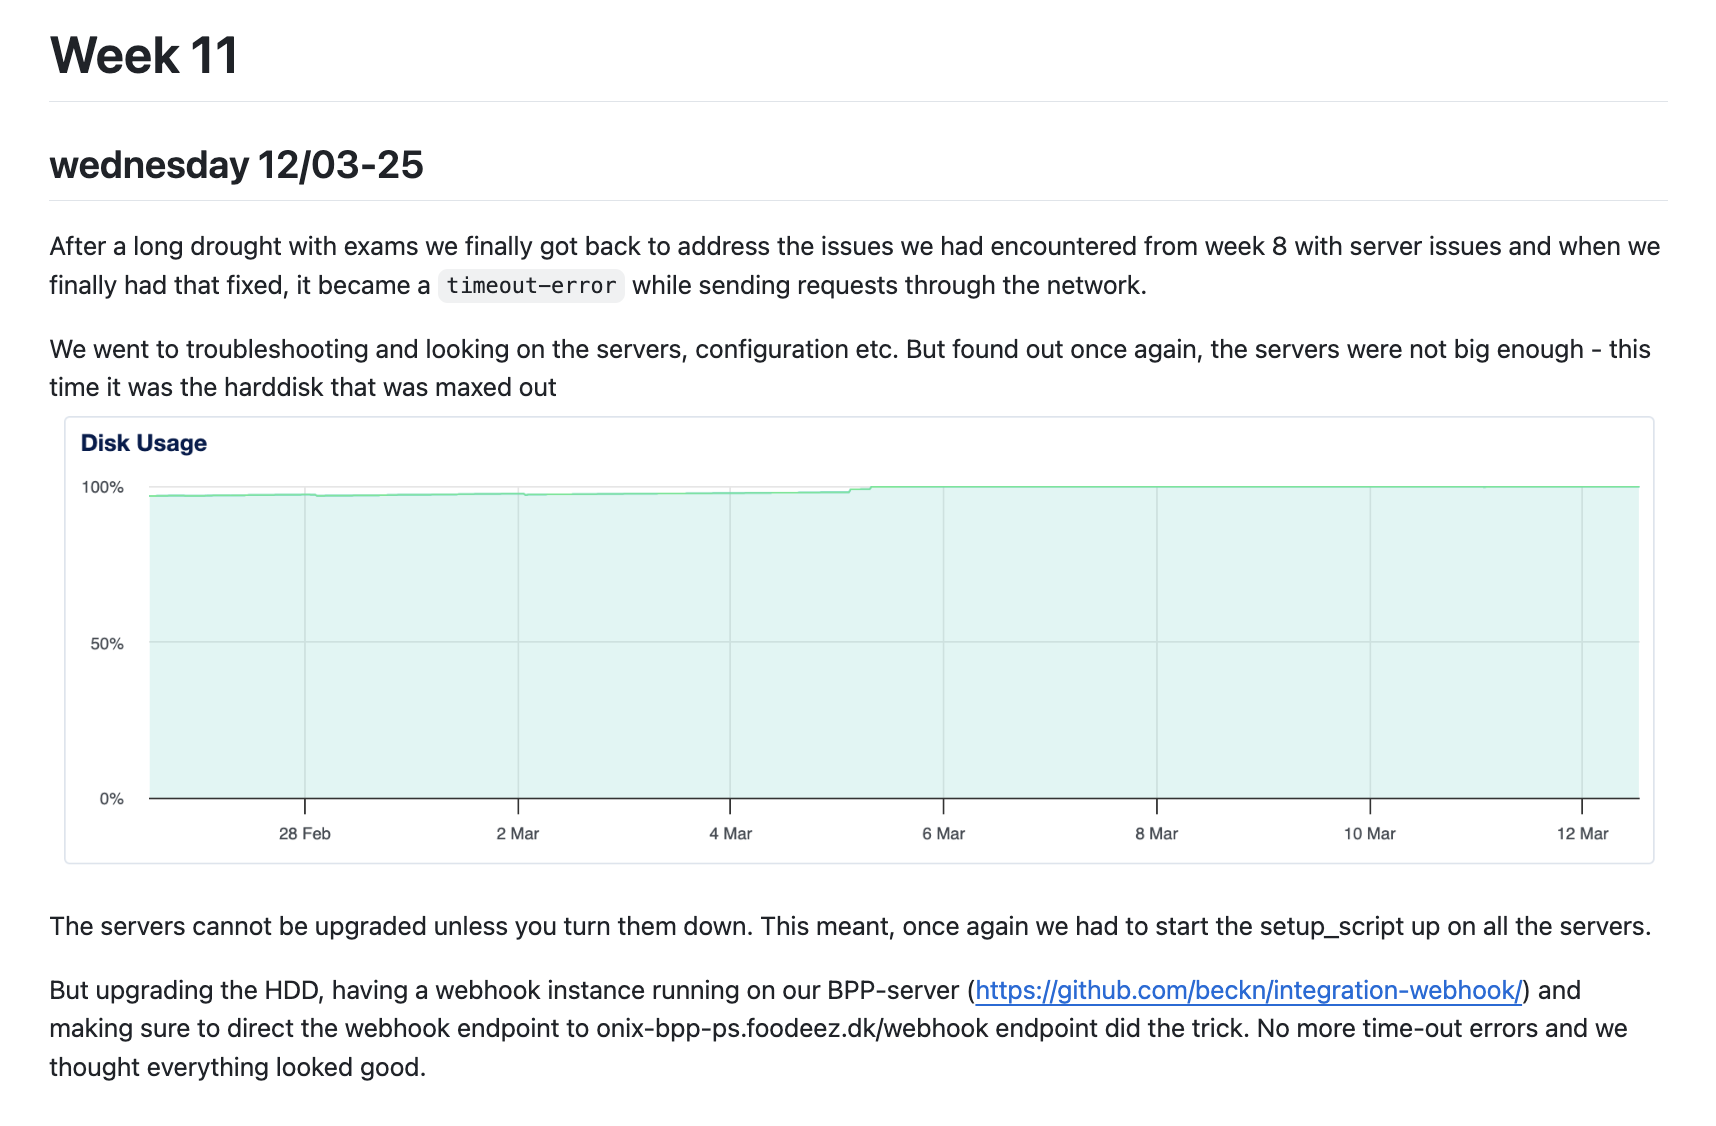
\includegraphics[width=\textwidth]{Images/week_11.png}
\end{figure}

\begin{figure}[H]
    \centering
    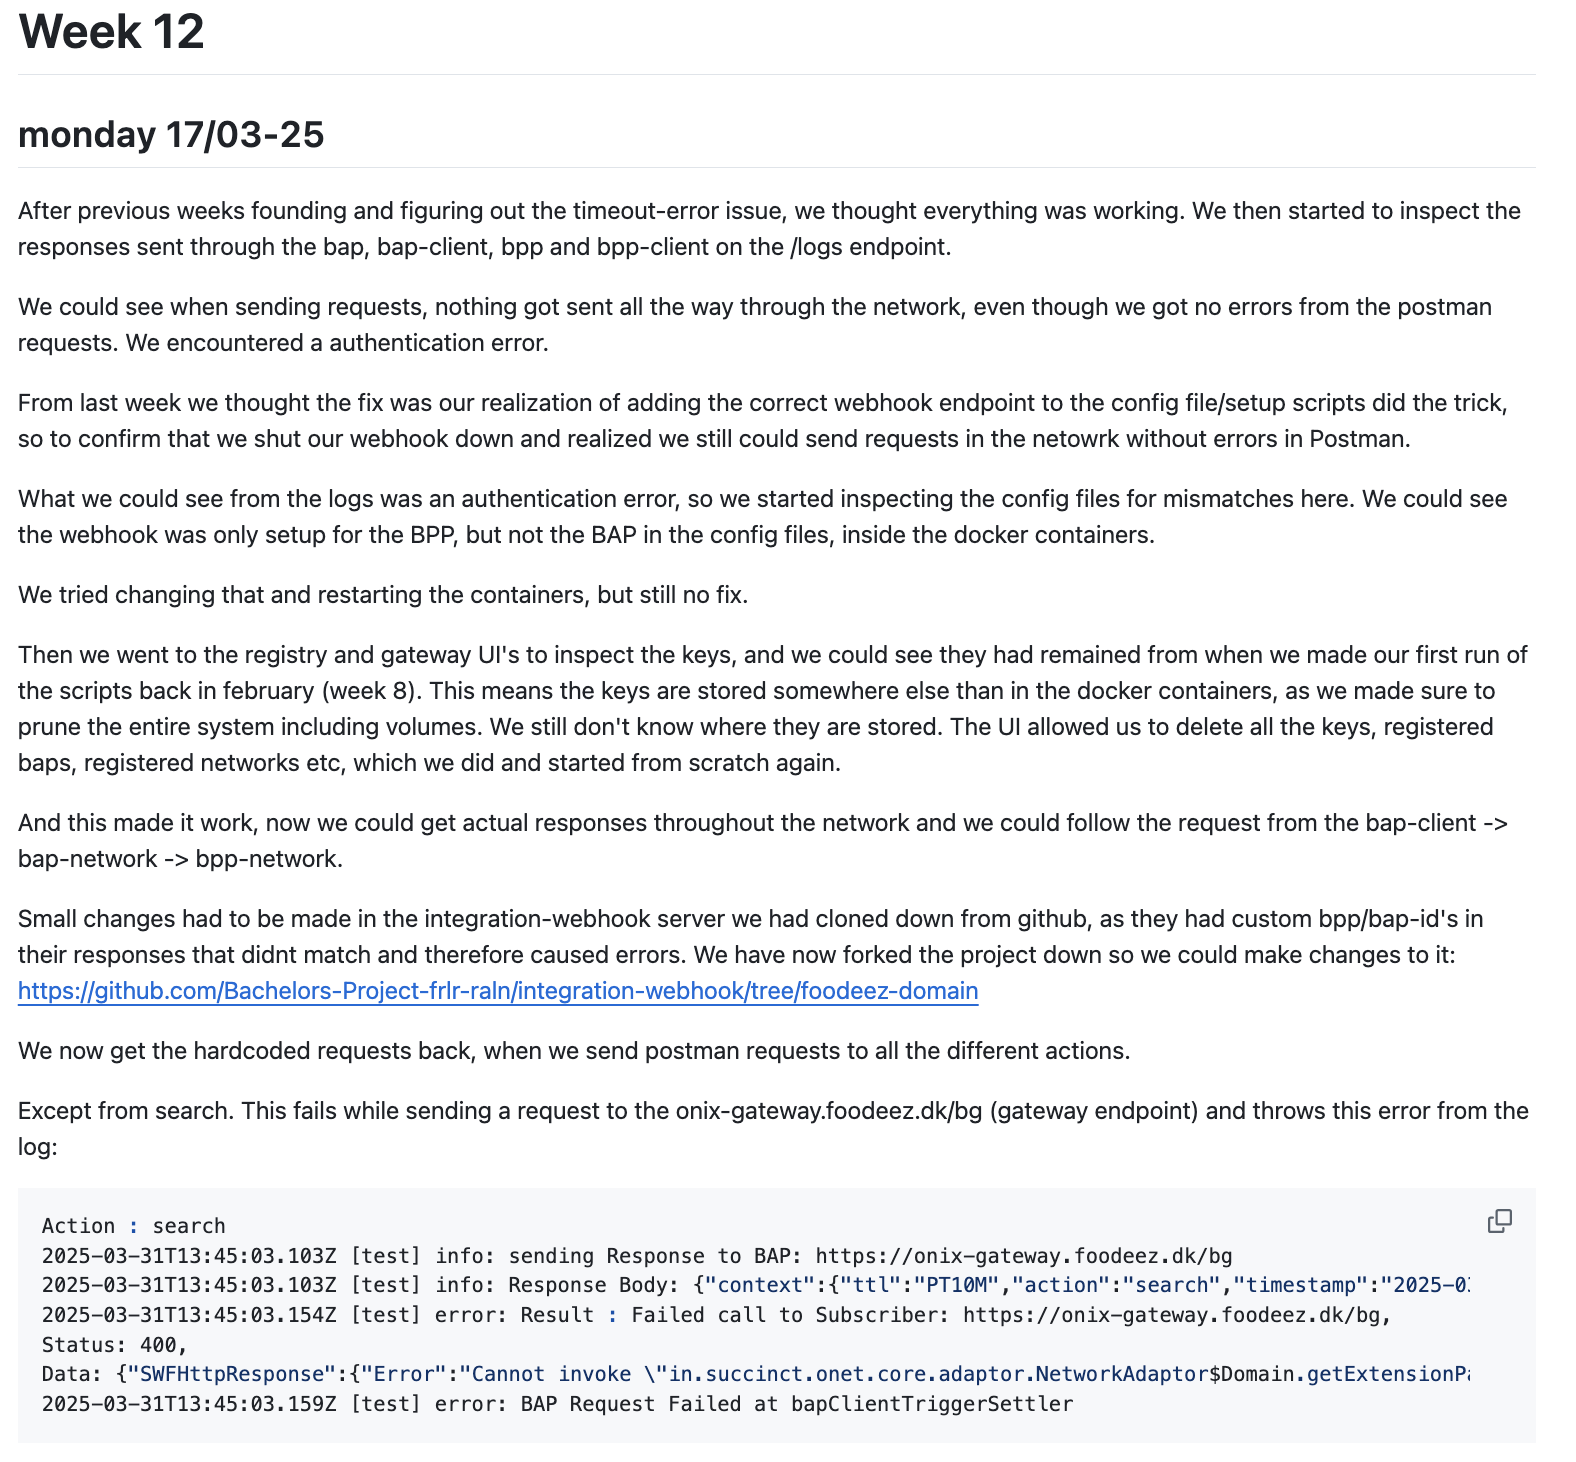
\includegraphics[width=\textwidth]{Images/week_12-13.png}
\end{figure}

\begin{figure}[H]
    \centering
    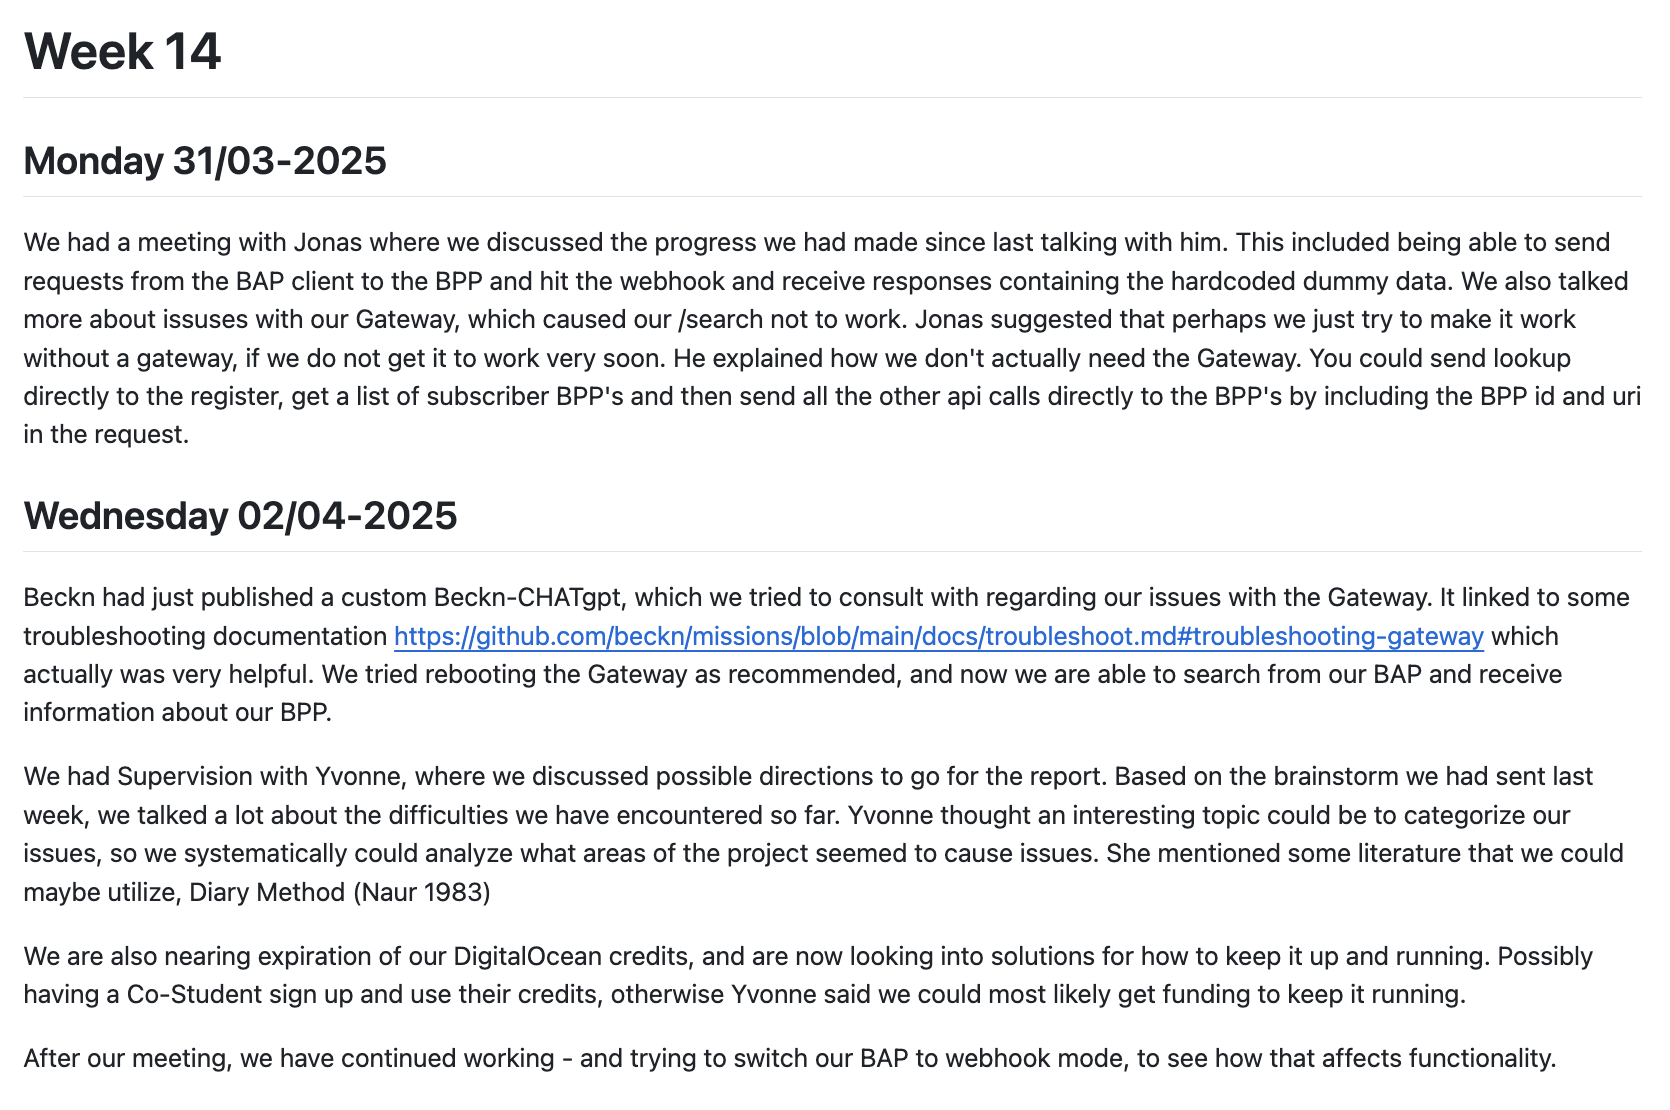
\includegraphics[width=\textwidth]{Images/week_14.png}
\end{figure}

\clearpage
\subsection{Beckn-IaC README} \label{readme_appendix}
\begin{figure}[h!]
    \centering
    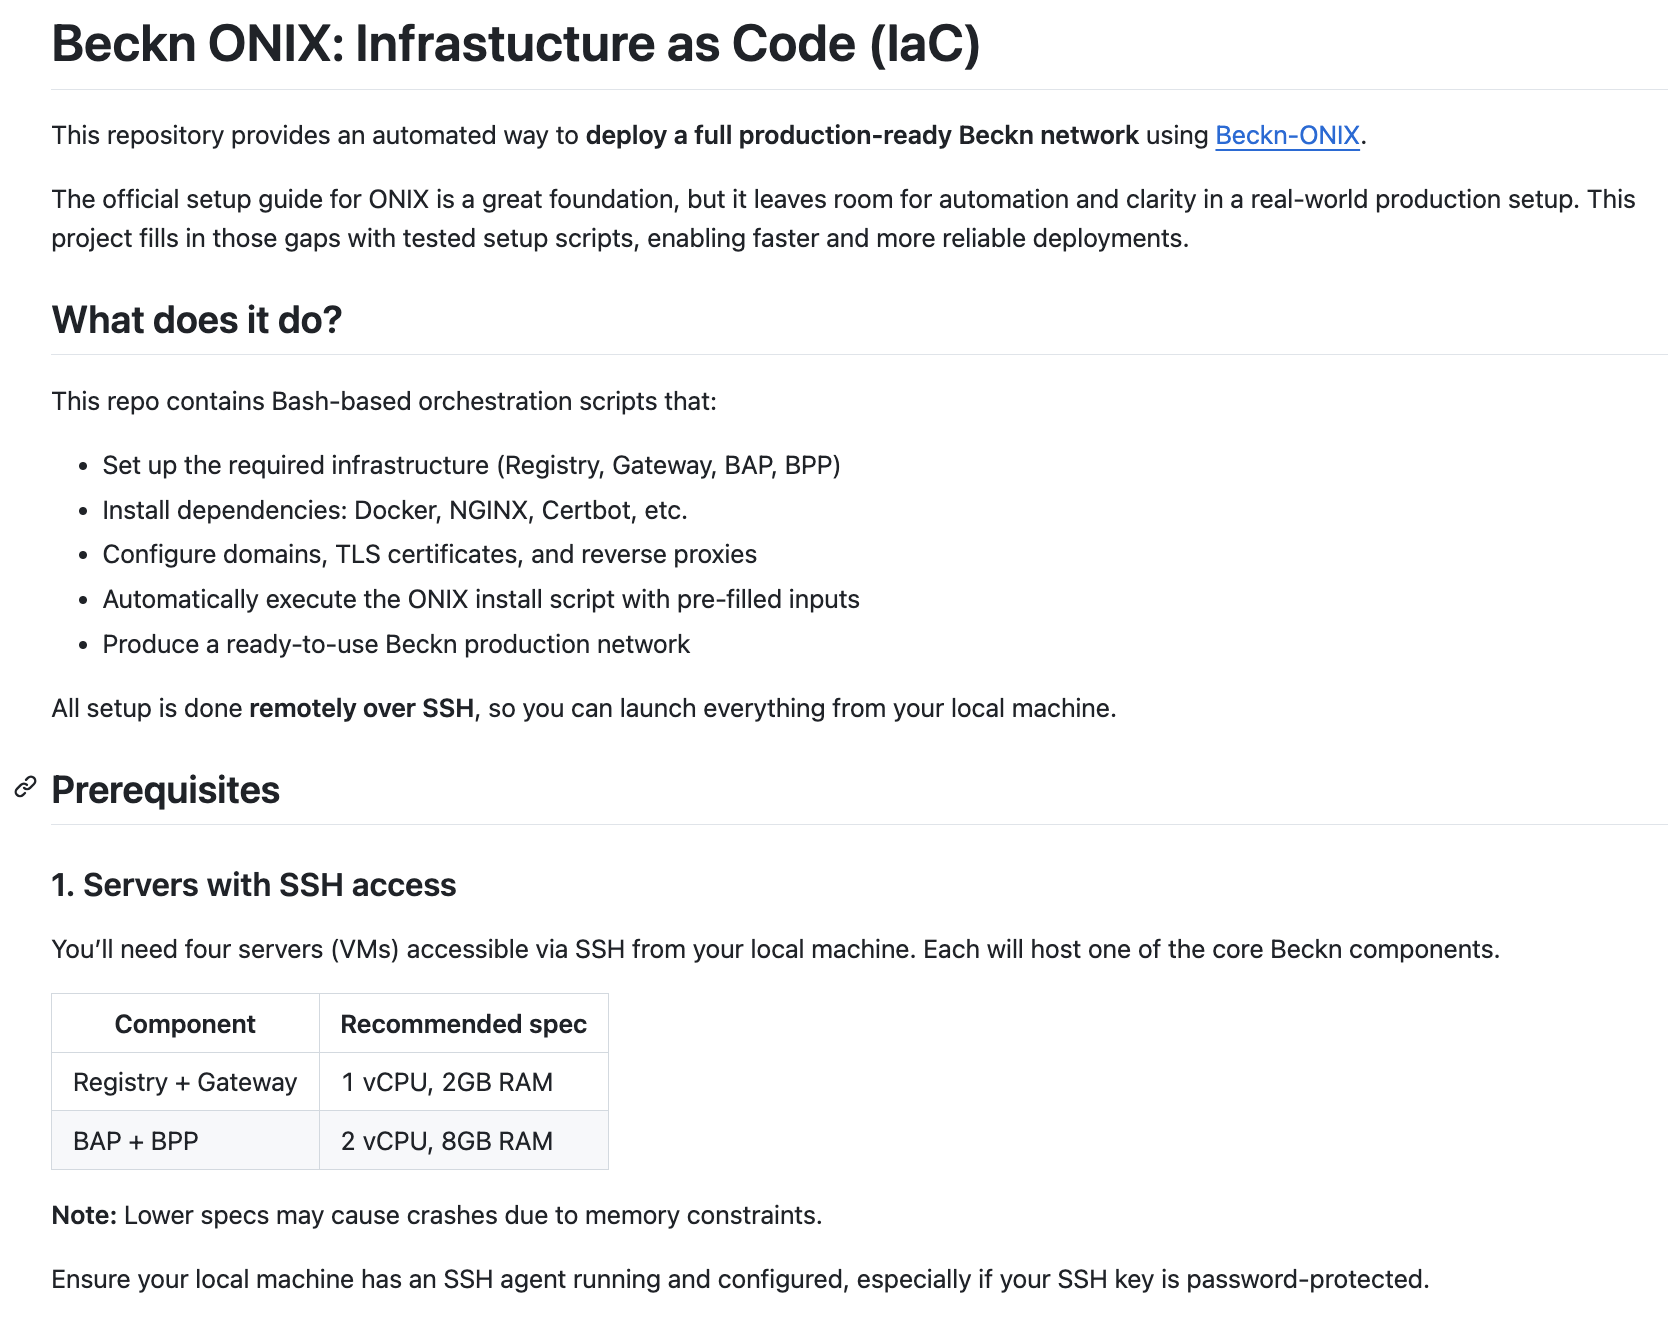
\includegraphics[width=1\textwidth]{Images/readme_1.png}
\end{figure}
\begin{figure}[h!]
    \centering
    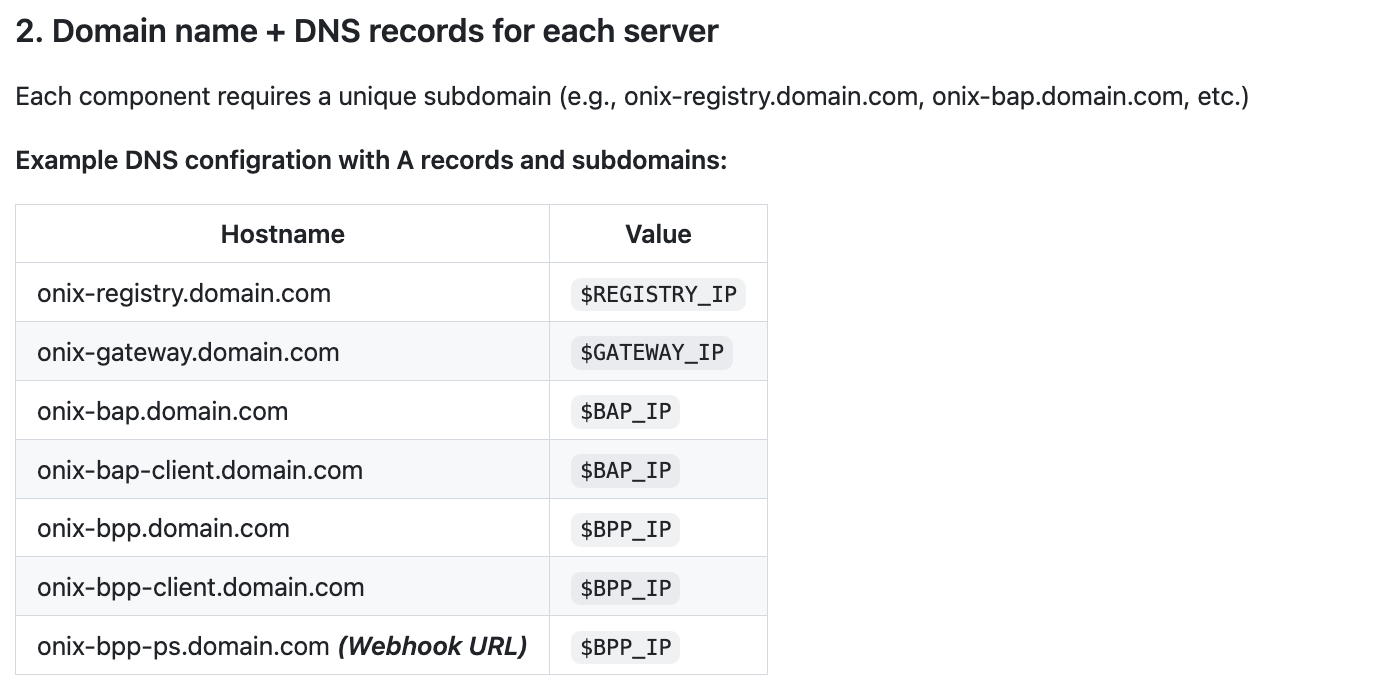
\includegraphics[width=1\textwidth]{Images/readme_2.png}
\end{figure}

\begin{figure}[h!]
    \centering
    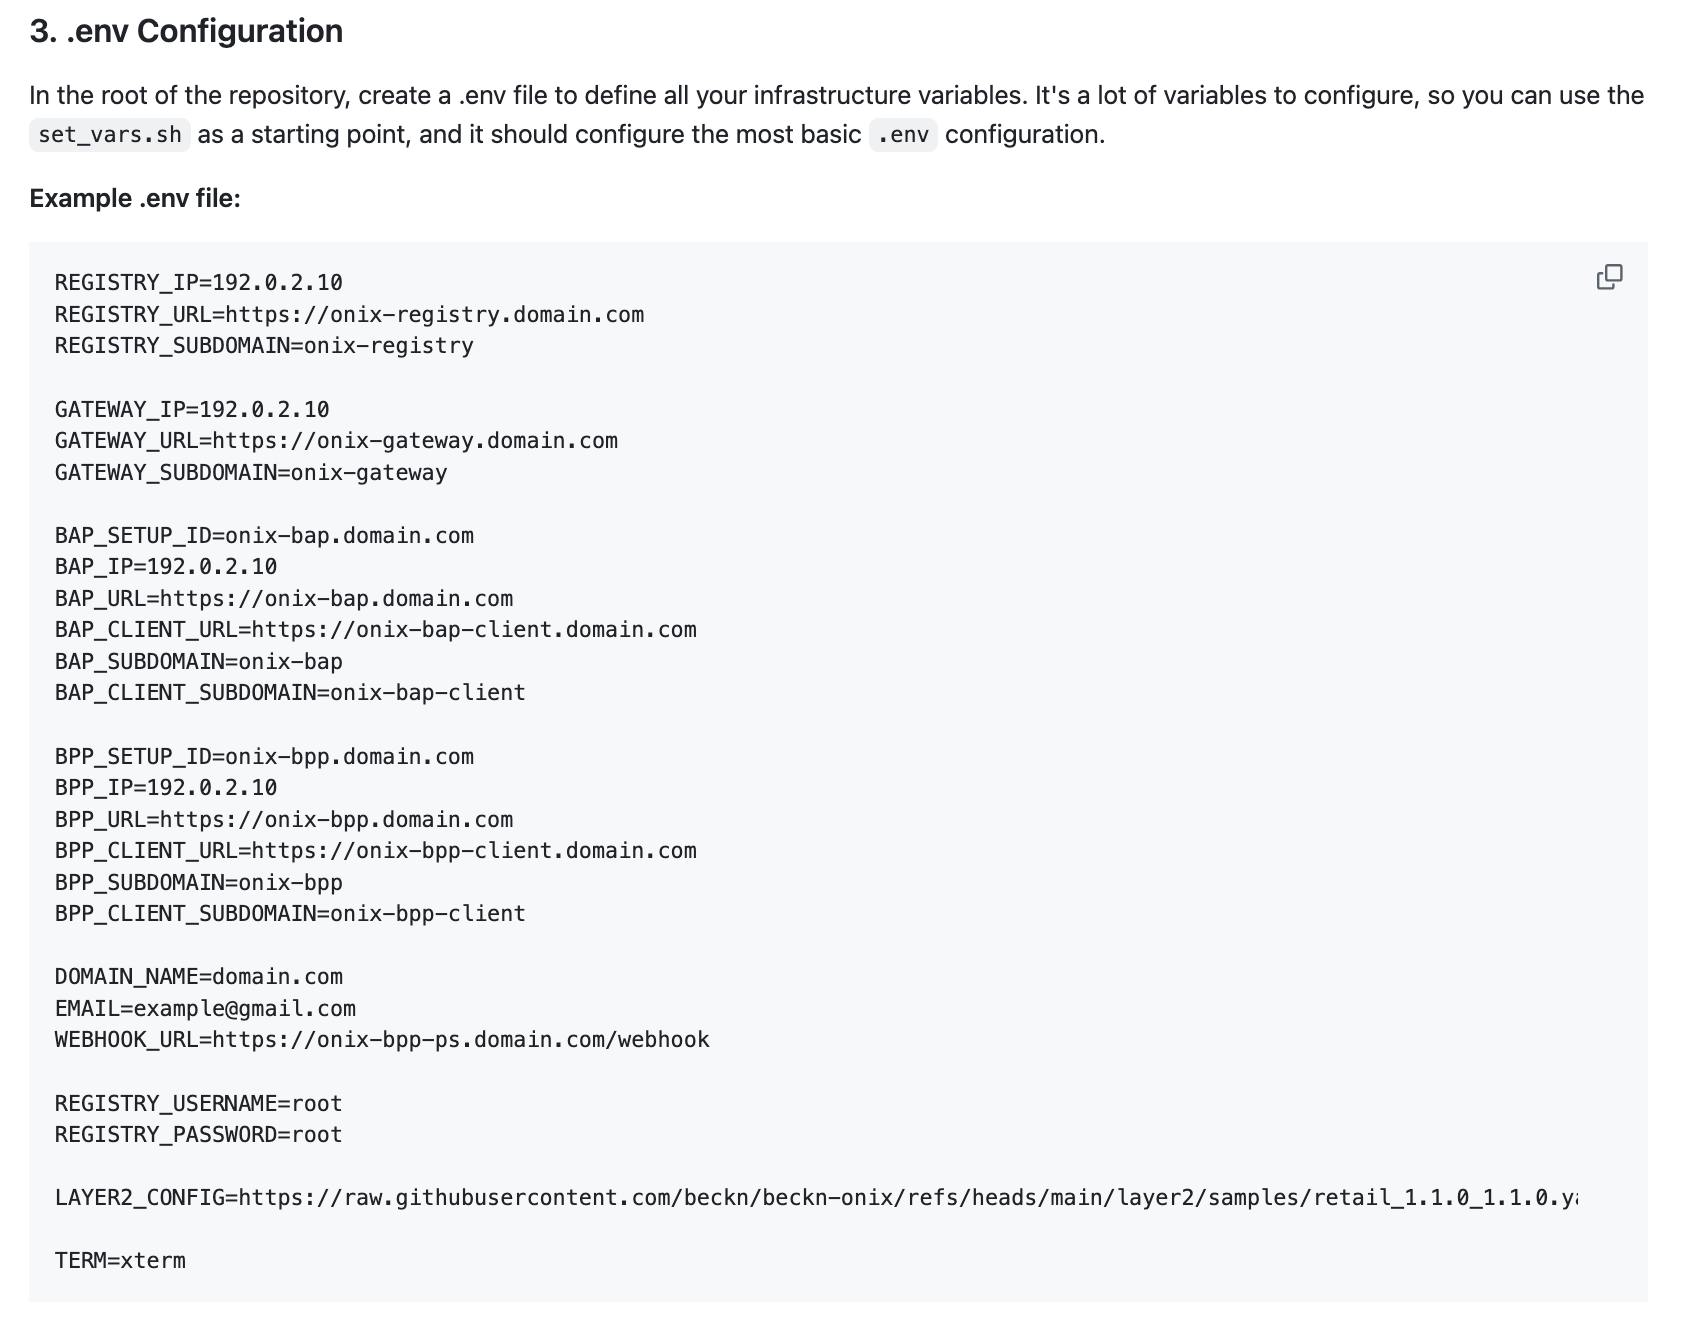
\includegraphics[width=1\textwidth]{Images/readme_3.png}
\end{figure}
\clearpage
\begin{figure}[h!]
    \centering
    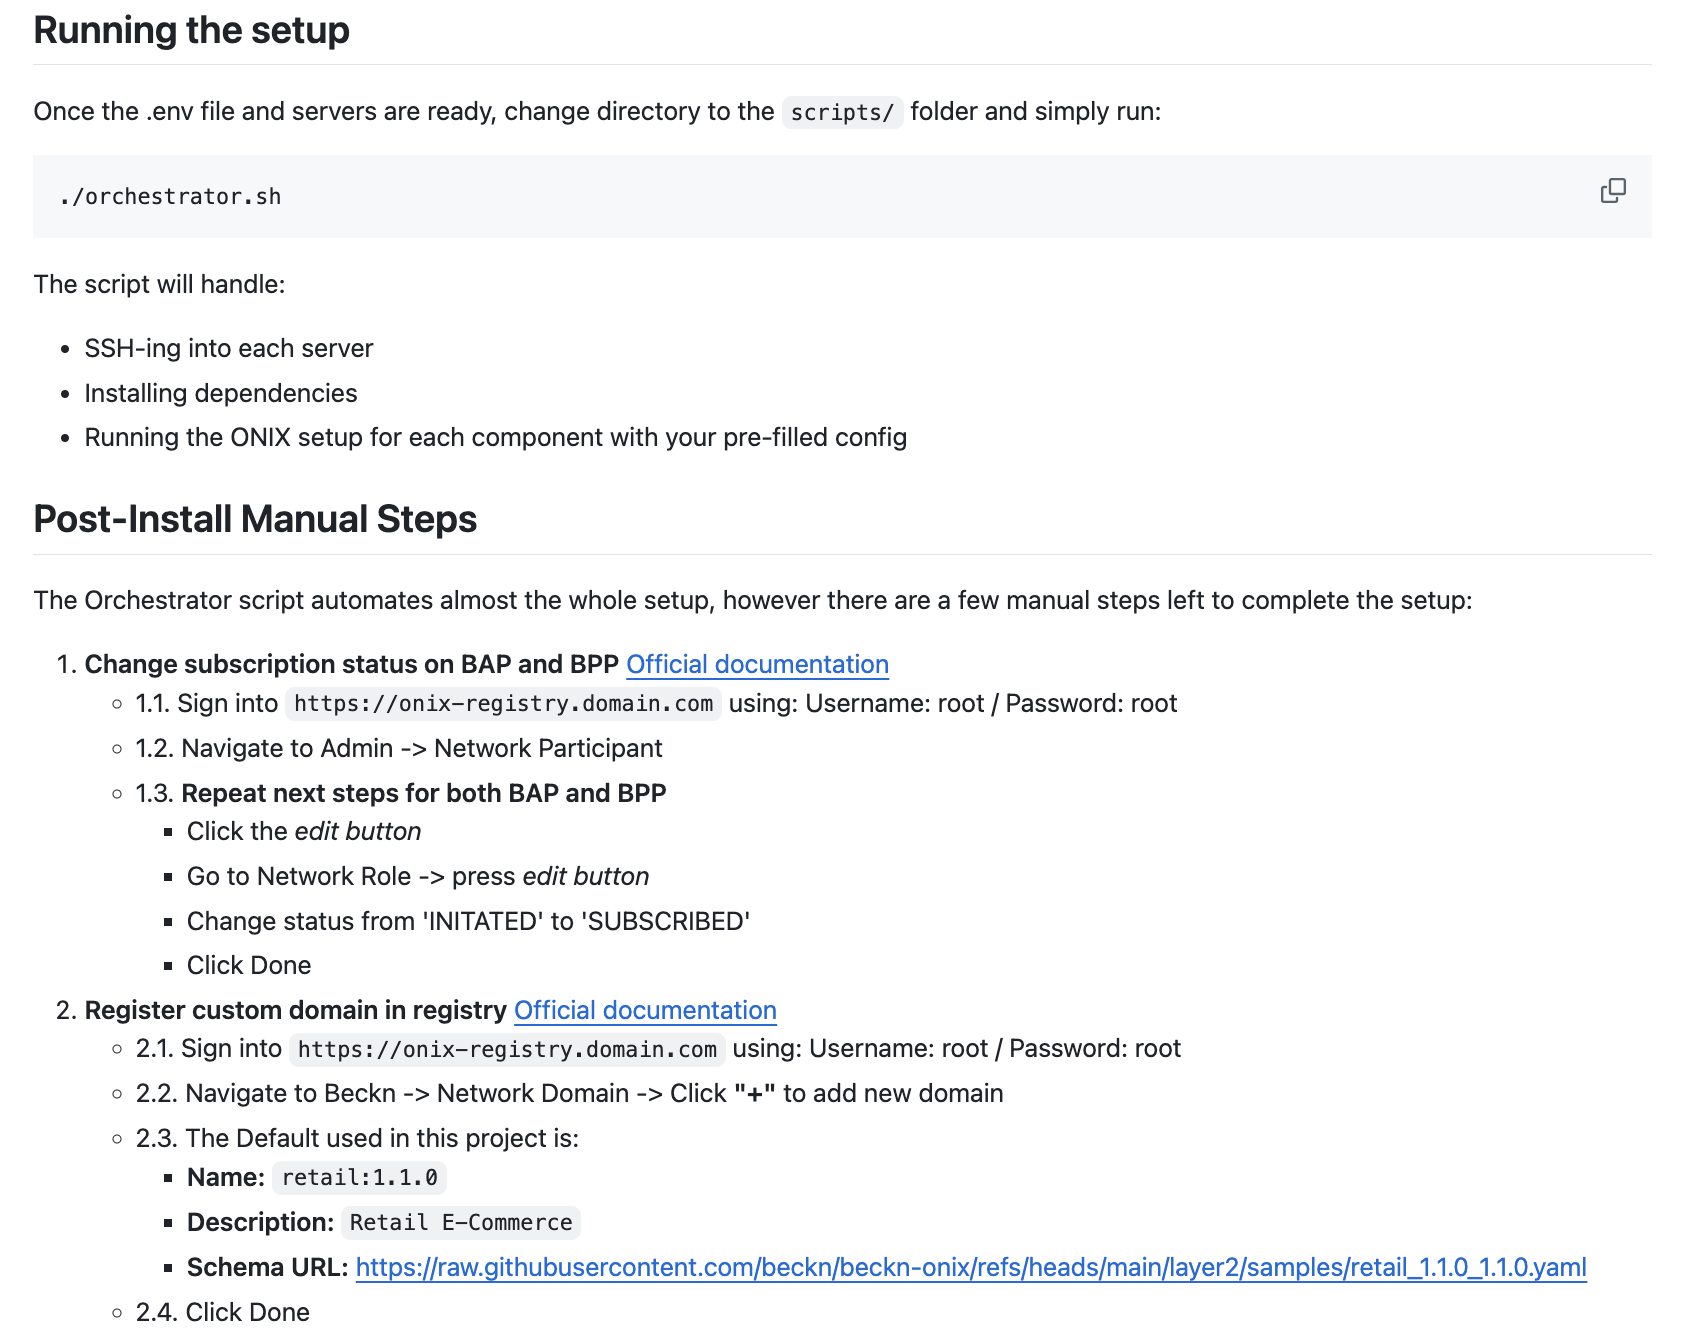
\includegraphics[width=1\textwidth]{Images/readme_4.png}
\end{figure}
\clearpage
\begin{figure}[h!]
    \centering
    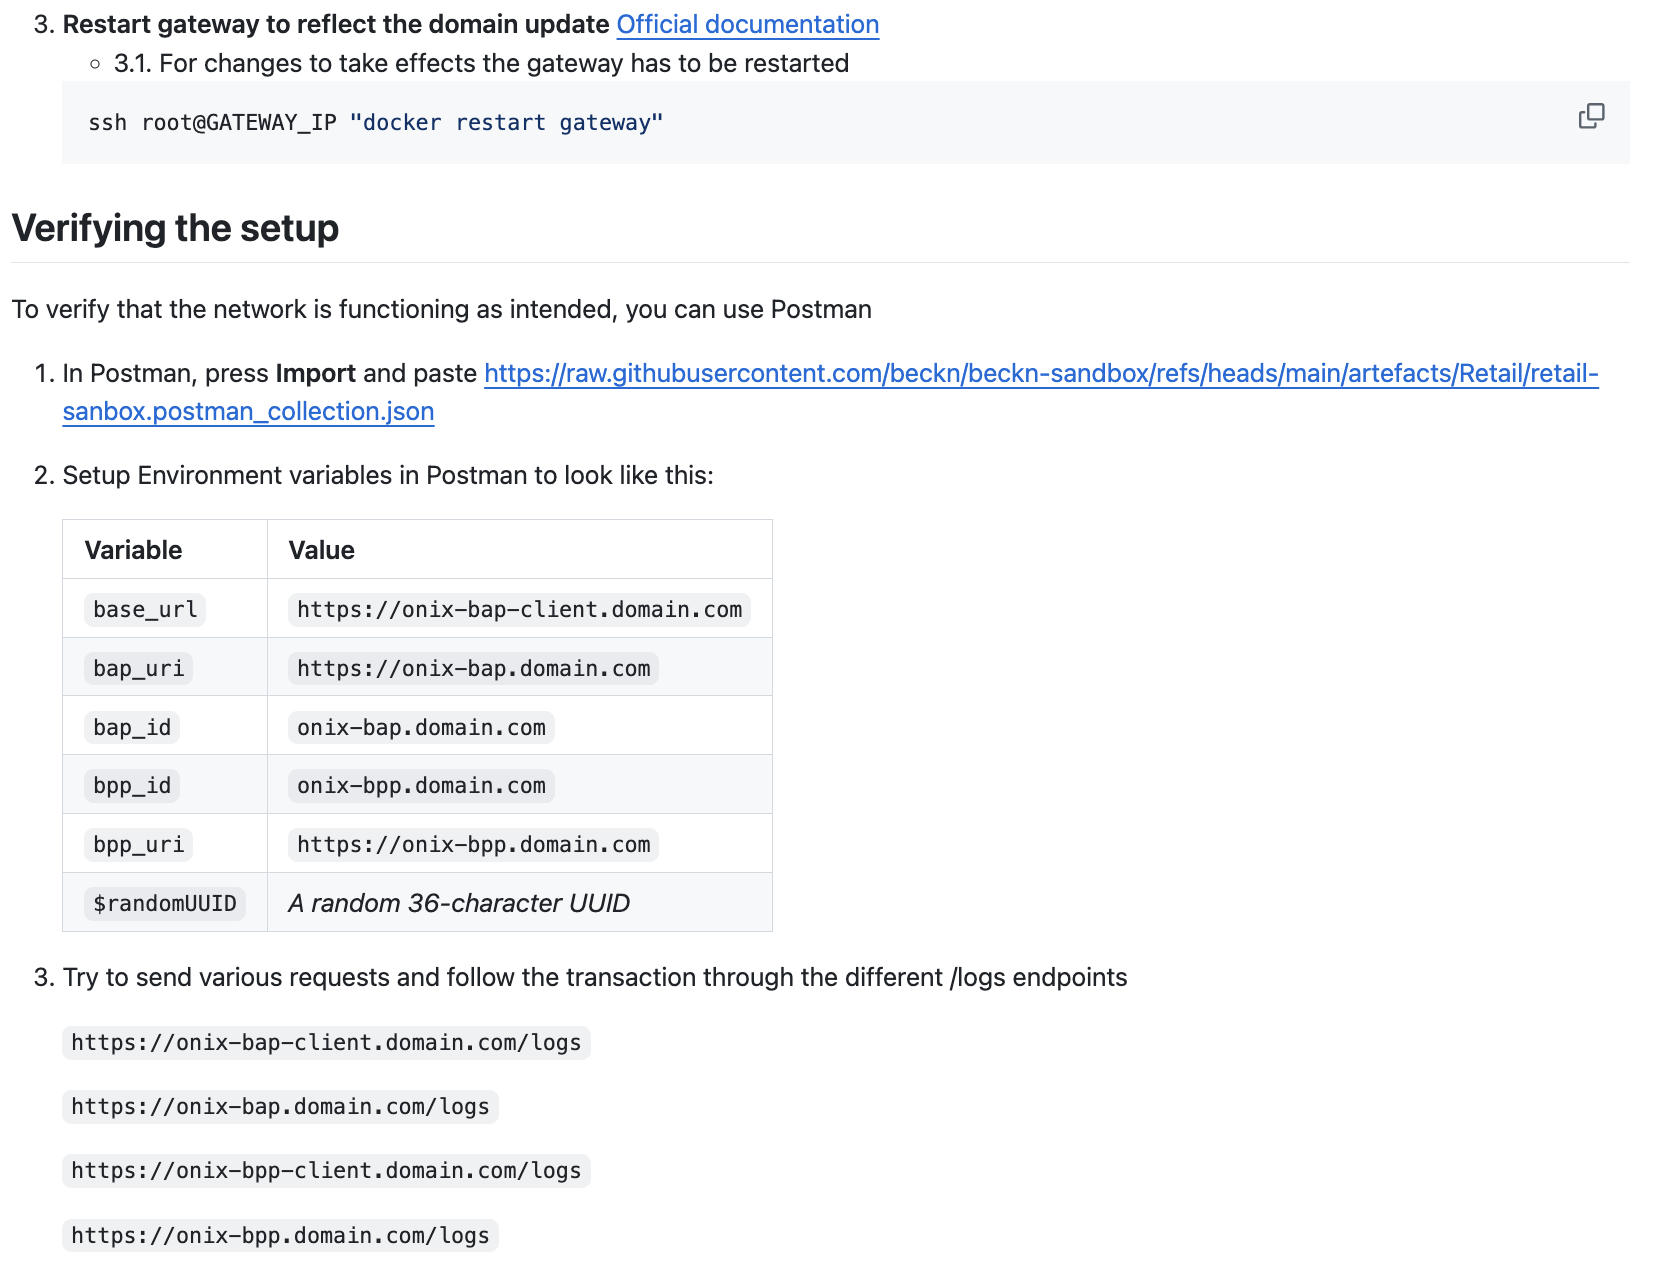
\includegraphics[width=1\textwidth]{Images/readme_5.png}
\end{figure}

\label{lastpage} % Last page label for references, pagenumber, etc.
